\clearpage
\appendix
\input{short_longitudinal}
\section{ITS Identity Theft Data Overview}
\label{app:demographics}


\subsection{Incident Characteristics}
\label{sec:incident_characteristics}

Next, summaries of the incidents affecting these victims were examined. The averages in Table \ref{tab:theft_summary_avg} represent the mean of the weighted survey values across the six survey years. It is important to note that for the "Type of Identity Theft" analysis, the percentages are calculated as a share of the total victim population for a given year. Because a single individual can experience multiple forms of identity theft (e.g., both credit card misuse and new account fraud), these categories are not mutually exclusive, and their percentages are not expected to sum to 100\%. Similarly, the percentages for the "How Misuse Was Discovered" and "How Information Was Obtained" sections do not total 100\%. This is because many respondents did not know the answer, and due to the skip logic of the survey. The questionnaire uses skip patterns, where a respondent's answer to one question determines whether they are asked subsequent, more detailed questions. For example, the question detailing the specific method of theft was only asked if a victim indicated that they knew how their information was obtained. If they answered "no," they were skipped past the follow up, and thus are not represented in any of those categories.

\begin{table}[h!]
  \centering
  \caption{Average Summary of Identity Theft Incidents (2008-2021).}
  \label{tab:theft_summary_avg}
  \begin{tabular}{lrr}
    \toprule
    \textbf{Category} & \textbf{N} & \textbf{\% of victims} \\
    \midrule
    \multicolumn{3}{l}{\textbf{Type of Identity Theft\tnote{*}}} \\
    \quad Existing Bank Account Misuse & 8,290,072 & 41.77 \\
    \quad Existing Credit Card Misuse & 9,476,109 & 48.23 \\
    \quad Other Existing Account Misuse & 2,598,402 & 12.28 \\
    \quad New Account Fraud & 1,443,137 & 7.82 \\
    \quad Other Misuse of Personal Information & 1,088,330 & 5.39 \\
    \quad Multiple Types & 2,734,282 & 13.76 \\
    \midrule
    \multicolumn{3}{l}{\textbf{How Misuse Was Discovered\tnote{**}}} \\
    \quad Noticed Problem with Account & 6,698,163 & 33.65 \\
    \quad Notified by Financial Institution & 7,790,053 & 37.69 \\
    \quad Notified by Other Person/Organization & 1,852,203 & 8.76 \\
    \quad Received Bill/Item Not Ordered & 679,982 & 3.63 \\
    \quad Checked Credit Report & 140,646 & 0.81 \\
    \quad Other/Unspecified & 1,807,364 & 8.37 \\
    \quad Unanswered/Not Applicable & 1,518,891\tnote{***} & 7.09 \\
    \midrule
    \multicolumn{3}{l}{\textbf{How Information Was Obtained\tnote{**}}} \\
    \quad Lost or Stolen Physical Item & 932,295 & 5.10 \\
    \quad Stolen During Transaction & 2,403,504 & 12.12 \\
    \quad Hacking/Computer Theft & 278,239 & 1.38 \\
    \quad Deceived by Scam/Phishing & 227,154 & 1.12 \\
    \quad Data Breach (Company/Employer) & 746,451 & 3.73 \\
    \quad Other & 574,991 & 2.67 \\
    \quad Unanswered/Not Applicable & 16,108,164\tnote{***} & 73.88 \\
    \bottomrule
  \end{tabular}
  % \begin{tablenotes}
  %   % \item[*] Categories are non-exclusive and may sum to more than 100\% as a single victim can experience multiple types of identity theft.
  %   % \item[**] The sum of percentages in these sections is approximately 100\% of the victim population.
  %   % \item[***] The Unanswered/Not Applicable row aggregates the weighted counts for respondents who were not asked the question due to survey skip logic or who had a missing data code (e.g., 'Don't Know' or 'Refused'). The values for 'Don't Know' were specifically filtered out of the listed categories and included here.
  % \end{tablenotes}
\end{table}
An analysis of Table \ref{tab:theft_summary_avg} verifies the trends discussed in \ref{app:longitudinal}. Table \ref{tab:theft_summary_avg} displays that on average, the misuse of existing accounts is the most common form of identity theft. Existing credit card misuse affected the largest share of victims (48.23\%), followed by the fraudulent use of existing bank accounts (41.77\%). These two categories alone demonstrate that the overwhelming majority of incidents involve the compromise of accounts that are already held by the victim. The creation of new fraudulent accounts and the misuse of personal information for other purposes, such as filing a fraudulent tax return, are notably less frequent, impacting 7.82\% and 5.39\% of victims, respectively. Furthermore, a significant portion of the victim population, 13.76\% on average, experienced more than one type of identity theft.

The most common methods by which victims discovered the fraud were being notified by a financial institution/bank (37.69\%), or personally noticing a problem with their account, such as not being able to make purchases anymore (33.65\%), which is a reflection of the prevalence and efficacy of fraud detection algorithms used by financial institutions. On the other hand, the proactive measure of checking credit reports was far less common in discovering misuse, with only 0.81\% of victims reporting that they discovered their incident in this way. Finally, Table \ref{tab:theft_summary_avg} shows that in terms of how the victims' personal information was obtained, no single method is dominant. The most frequently cited pathway was information being stolen during a transaction, either online or in-person, accounting for 12.12\% of incidents. Interestingly, while digital threats are a major public concern, direct hacking or computer theft was reported in only 1.38\% of cases, and data breaches from companies or employers accounted for just 3.73\% on average. It is also noteworthy that traditional, non-digital methods remain relevant. For example, 5.10\% of incidents resulted from a lost or stolen physical item, such as a wallet or mail. However, all these values only reflect the victims who knew how their information was obtained. The vast majority of victims did not know, therefore these statistics may not be an accurate reflection of how the information of most victims was obtained.
%\com{This is purely optional, but some of the stats reporting could be presented in enumeration/bullet form, may make it a bit easier to read..}





\subsection{Summary of Data Demographics}

Recall that Table \ref{tab:victimization_year} showed that the number of identity theft victims has been generally increasing with each survey wave. While identity theft affects all segments of the population, comparison of the data sample's victimization with U.S. Census data reveals some disparities in victimization risk, detailed in Table \ref{tab:demographics_percent} in Appendix \ref{app:demographics_census}. Specifically, victims aged 30-64 are overrepresented among victims. Additionally, white individuals are overrepresented among victims, while  individuals of Black, Asian, American Indian or Alaskan Native descent, or of two or more races, are all underrepresented among victims. On the impact of education level, individuals with a Bachelor's degree or a Graduate/Professional degree are overrepresented among victims. Similar to education, with respect to income, households earning \$75,000 and over are the most victimized group, being slightly overrepresented compared to their share of the population. Households in the lower income brackets (\$25,000 or less) are underrepresented among victims. 

To further investigate why certain groups are disproportionately represented, we conducted a series of deeper analyses, including weighted proportions tests and logistic regressions, extending the work of \cite{Reynolds2021Differential, DeLiema2021} to all six waves of the ITS survey. Our results are detailed in \ref{app:demographics_census} and in the extended version \cite{Anonymous2026SocialCostExtended}, and are summarized as follows. First, we found that victims aged 30-64 are ``digitally active but not digitally native,'' meaning that they are significantly more vulnerable to digital theft than the 16-29 ``digital native'' group. Next, we found disparities in the specific types of fraud experienced across different demographics. Our analysis in the extended version \cite{Anonymous2026SocialCostExtended} reveals that the over-representation of White and highly educated victims is primarily driven by existing credit card misuse, aligning with the results of \cite{Nevin2025, Copes2010}. It was also found that Black individuals and lower-SES groups are disproportionately victimized by more invasive forms of identity theft, such as existing bank account and new account fraud. For example, we found that Black victims report existing bank account misuse at a rate higher than the White victim population, a finding that aligns with prior research on target suitability and financial accessibility \cite{Copes2010}. Finally, the results of our regression analysis in the extended version \cite{Anonymous2026SocialCostExtended} verified the trends described in \cite{Reynolds2021Differential}, where higher levels of age, education, and income increase the odds of identity theft victimization. Thus, the trends observed in previous studies using a fraction of ITS surveys continue to be observed when all six waves are pooled.
%\com{Do any of these observations appear more or less  pronounced/subdued than previously observed, and are there new observations..?}
%\resp{I'm not so sure how to compare them, since their analyses were slightly different than ours, so I can't compare the odds ratios.}

%%%%%%%%%%%%%%%%%%%%%


\section{Detailed Data Demographics and Census Comparison}
\label{app:demographics_census}

Here we display a set of descriptive statistics for the combined dataset,  shown in Table \ref{tab:demographics_percent}, which provides an averaged demographic profile of victims and juxtaposes it against data for the general U.S. population from the Census Bureau. The Victim \% column reflects the characteristics of the sample of 41,091 victims from the harmonized data. To achieve this, the survey weights for victims within a specific category (for example, those aged 30-49 or holding a Bachelor's degree) were summed and then divided by the total weighted victim population. The result is an averaged demographic of a typical identity theft victim between 2008 and 2021. 

For the Census \% column, data was aggregated from several U.S. Census Bureau surveys corresponding to the ITS years (2008, 2012, 2014, 2016, 2018, and 2021). Race data was sourced from the American Community Survey (ACS) 1-Year Data Profile DP05 \cite{Census_ACS_DP05}, while household income data came from the Current Population Survey's (CPS) Table H-17 \cite{Census_CPS_H17}. The remaining categories of age, sex, and educational attainment were derived from ACS tables on U.S. age and sex composition \cite{Census_AgeSex}. The final percentages represent the average demographic makeup of the U.S. population across these years. Note that in this process, age related categories were aligned to ensure a valid comparison, because the ITS sample includes only individuals aged 16 or older. Thus, because ACS groups individuals aged 15-19, a proportional allocation of 80\% or four fifths of this group was used to estimate the 16-19 population. A similar adjustment was made for the educational attainment data where a 15-17 age bracket appeared, and two thirds of that population was taken to estimate the count for ages 16-17. 

\begin{longtable}{lrr}
\caption{Comparison of victim demographics to Census data (\%), averaged over 2008-2021.} \label{tab:demographics_percent} \\
\toprule
\textbf{Category} & \textbf{Victim \%} & \textbf{Census \%} \\
\midrule
\endfirsthead
\multicolumn{3}{c}%
{{\tablename\ \thetable{} -- continued from previous page}} \\
\toprule
\textbf{Category} & \textbf{Victim \%} & \textbf{Census \%} \\
\midrule
\endhead
\midrule
\multicolumn{3}{r}{{Continued on next page}} \\
\endfoot
\bottomrule
\endlastfoot
\multicolumn{3}{c}{\textbf{Age Group}} \\
\midrule
16-29 & 18.03 & 24.35 \\
30-49 & 38.25 & 33.32 \\
50-64 & 28.14 & 24.44 \\
65+ & 15.58 & 17.89 \\
\midrule
\multicolumn{3}{c}{\textbf{Victim Sex}} \\
\midrule
Male & 47.43 & 47.73 \\
Female & 52.57 & 52.27 \\
\midrule
\multicolumn{3}{c}{\textbf{Victim Race/Ethnicity}} \\
\midrule
White alone & 81.96 & 75.3 \\
Black or African American alone & 10.35 & 13.2 \\
Asian alone & 4.96 & 5.5 \\
American Indian/Alaska Native alone & 0.62 & 0.9 \\
Native Hawaiian/Pacific Islander alone & 0.29 & 0.2 \\
Two or More Races & 1.83 & 4.9 \\
\midrule
\multicolumn{3}{c}{\textbf{Victim Educational Attainment}} \\
\midrule
Less than High School & 5.60 & 15.17 \\
High School Graduate (or equivalent) & 18.12 & 28.38 \\
Some College/Associate Degree & 30.16 & 27.18 \\
Bachelor's Degree & 28.10 & 18.87 \\
Graduate/Professional Degree & 18.02 & 10.38 \\
\midrule
\multicolumn{3}{c}{\textbf{Victim Household Income}} \\
\midrule
Under \$15,000 & 5.78 & 8.32 \\
\$15,000 to \$24,999 & 5.46 & 7.95 \\
\$25,000 to \$49,999 & 19.92 & 19.12 \\
\$50,000 to \$74,999 & 18.26 & 15.78 \\
\$75,000 and over & 50.58 & 48.90 \\
\end{longtable}

As mentioned earlier, Table \ref{tab:demographics_percent} provides several insights about the differences between the demographic profile of a victim versus the entire population. For example, adults aged 30-49 and 50-64 are overrepresented among victims compared to their share of the general population. Younger individuals aged 16-29 and seniors aged 65+ are underrepresented. This could suggest that identity theft disproportionately affects individuals who are in their prime working and earning years. On the other hand, victimization rates between sexes are remarkably aligned with the national population, suggesting that sex is not a significant differentiating factor in identity theft victimization. 

Table \ref{tab:demographics_percent} also highlights disparities in victimization rates across racial lines. White individuals are overrepresented among victims, making up 82\% of the victim population but only 75\% of the general population. In contrast, individuals of Black, Asian, American Indian or Alaskan Native descent, or of two or more races, are all underrepresented among victims. It is also noticeable that individuals with a Bachelor's degree or a Graduate/Professional degree are overrepresented among victims. For example, those with a graduate degree make up over 18\% of victims but only about 10\% of the census population. Those with a High school education or less are significantly underrepresented among victims. The impact of income is also shown, where households earning \$75,000 and over are slightly overrepresented, and  households in the lower income brackets (\$25,000 or less) are underrepresented. As mentioned earlier, these disparities are further explored in the extended version, \cite{Anonymous2026SocialCostExtended}.



% \section{Imputation of Undisclosed Records}
% \label{app:imputation_nu}

% To ensure the continuity of the data breach chronology, we addressed the volume of incidents lacking disclosed record counts by calculating an annual baseline number of undisclosed records, $n_u$. 




\section{Inflation Adjustments}
\label{app:inflation}
The formula used to convert a nominal monetary value from a given year to its real value in 2021 dollars is as follows:
\begin{equation}
\label{eq:inflation_adjustment}
\text{Adjusted Value (in 2021 \$)} = \text{Nominal Value} \times \left( \frac{\text{CPI}_{2021}}{\text{CPI}_{\text{Original Year}}} \right)
\end{equation}

Table \ref{tab:appendix_cpi} displays all the CPI values that were used for these calculations. This inflation adjustment was applied to any monetary value in this paper. These CPI values were obtained from the U.S. Bureau of Labor Statistics \cite{BLS_CPI, USInflationCalc_CPI}.

\begin{table}[ht]
\centering
\caption{Annual Average Consumer Price Index (CPI)}
\label{tab:appendix_cpi}
\begin{tabular}{lr}
\toprule
\textbf{Year} & \textbf{Annual Average CPI} \\
\midrule
2008 & 215.297 \\
2012 & 233.165 \\
2014 & 236.736 \\
2016 & 240.007 \\
2018 & 251.107 \\
2021 & 270.970 \\
% 2023 & 304.702 \\
% 2024 & 313.689 \\
\bottomrule
\end{tabular}
\end{table}

\section{Average Private Nonfarm Hourly Wages}
\label{app:hourly_wages}
To estimate opportunity cost of lost time in the social cost calculations, time lost was multiplied by the respective year's average hourly wage, shown in Table \ref{tab:appendix_wage}. This private nonfarm hourly wage data represents the vast majority of the U.S. workforce, and was obtained from \cite{FRED_Wage}.

\begin{table}[ht]
\centering
\caption{Nominal and Inflation-Adjusted Average Private Hourly Wage}
\label{tab:appendix_wage}
\begin{tabular}{lrr}
\toprule
\textbf{Year} & \multicolumn{2}{c}{\textbf{Average Private Hourly Wage}} \\
\cmidrule(lr){2-3} % Draws a line under columns 2 and 3 only
& \textbf{Nominal} & \textbf{Adjusted} \\
\midrule
2008 & 21.19 & 26.67 \\
2012 & 23.26 & 27.03 \\
2014 & 24.23 & 27.73 \\
2016 & 25.37 & 28.64 \\
2018 & 26.72 & 28.83 \\
2021 & 29.92 & 29.92 \\
\bottomrule
\end{tabular}
\end{table}

\section{Fixed Service Costs for Social Cost Calculations}
\label{app:fixed_service_costs}
To estimate the cost of hiring a lawyer, a doctor or therapy appointment, or obtaining medication, we constructed the following Table \ref{tab:appendix_cost_estimates_sourced}, where costs were also adjusted for inflation.

\begin{table}[ht]
\centering
\caption{Cost Estimates and Sources for Social Cost Calculations}
\label{tab:appendix_cost_estimates_sourced}
\small % Using a smaller font size to help the table fit
\begin{tabular}{l l r c r l l}
\toprule
\thead{Item} & 
\thead{Reported \\ Nominal Cost} & 
\thead{Assumed \\ Nominal \\ Cost (\$)} & 
\thead{Source \\ Year} & 
\thead{Adjusted \\ Cost \\ (2021 \$)} & 
\thead{Notes} &
\thead{Source} \\
\midrule
Lawyer & \$327 per hour & 500 & 2023 & 444.65 & Based on approx. 1.5 hours & \cite{USNews_Lawyer}\\
Doctor Visit & \$79--172 & 100 & 2024 & 86.38 & Without insurance & \cite{DebtOrg_Doctor} \\
Therapist Visit & \$100--200 & 100 & 2024 & 86.38 & Without insurance & \cite{GoodRx_Therapy} \\
Medication & \$50 & 50 & 2018 & 53.96 & Generic prescription & \cite{CBO_Prescription} \\
\bottomrule
\end{tabular}
\end{table}


\section{ITS Victim Timeline}
\label{app:timeline}
To plot the number of reported identity thefts per month from the ITS dataset, the following assumptions were made. The primary variable used for the timeline is the month in which the victim first discovered the identity theft. For survey years where this specific "discovery month" was explicitly recorded (such as the redesigned 2021 ITS), that value was used directly. For survey waves or individual records where a specific discovery month was missing or not collected, the month was estimated using the Interview Quarter variable. In cases where only the interview quarter was available, incidents were mapped to the mid-month of that quarter to provide a representative point estimate (e.g., Quarter 1 $\rightarrow$ February, Quarter 2 $\rightarrow$ May, Quarter 3 $\rightarrow$ August, Quarter 4 $\rightarrow$ November). This ensures the timeline reflects the general seasonal distribution of reports while acknowledging the six-month reference period typically used in the NCVS core interview. Monthly counts were calculated by summing the final ITS weights of all confirmed victims discovered or reported in that month. This allows the timeline to represent national-level estimates of identity theft discovery rather than raw sample counts.

% Finally, since the ITS is typically administered every two years and often for only six-month field periods, the resulting monthly series contains gaps between survey waves. To create a continuous timeline for comparison with external data breaches, a log-linear interpolation was applied to smooth these transitions and estimate the latent victim count during non-survey months.

\section{Dynamic Saturation Model}
\label{app:sat_model}
Here we display the month-to-month overlay and conversion rate results, as well as Wilcoxon signed-rank testing results, for the output of our dynamic saturation model with $Y=15$ (proposed in Section \ref{sec:estimating_number_records}). Recall that the purpose of this model is to take the augmented PRC data as an input, and output the estimated number of unique individuals whose data was compromised.

\begin{figure}[htbp]
    \centering
    % First Figure
    \begin{minipage}[t]{0.32\textwidth}
        \centering
        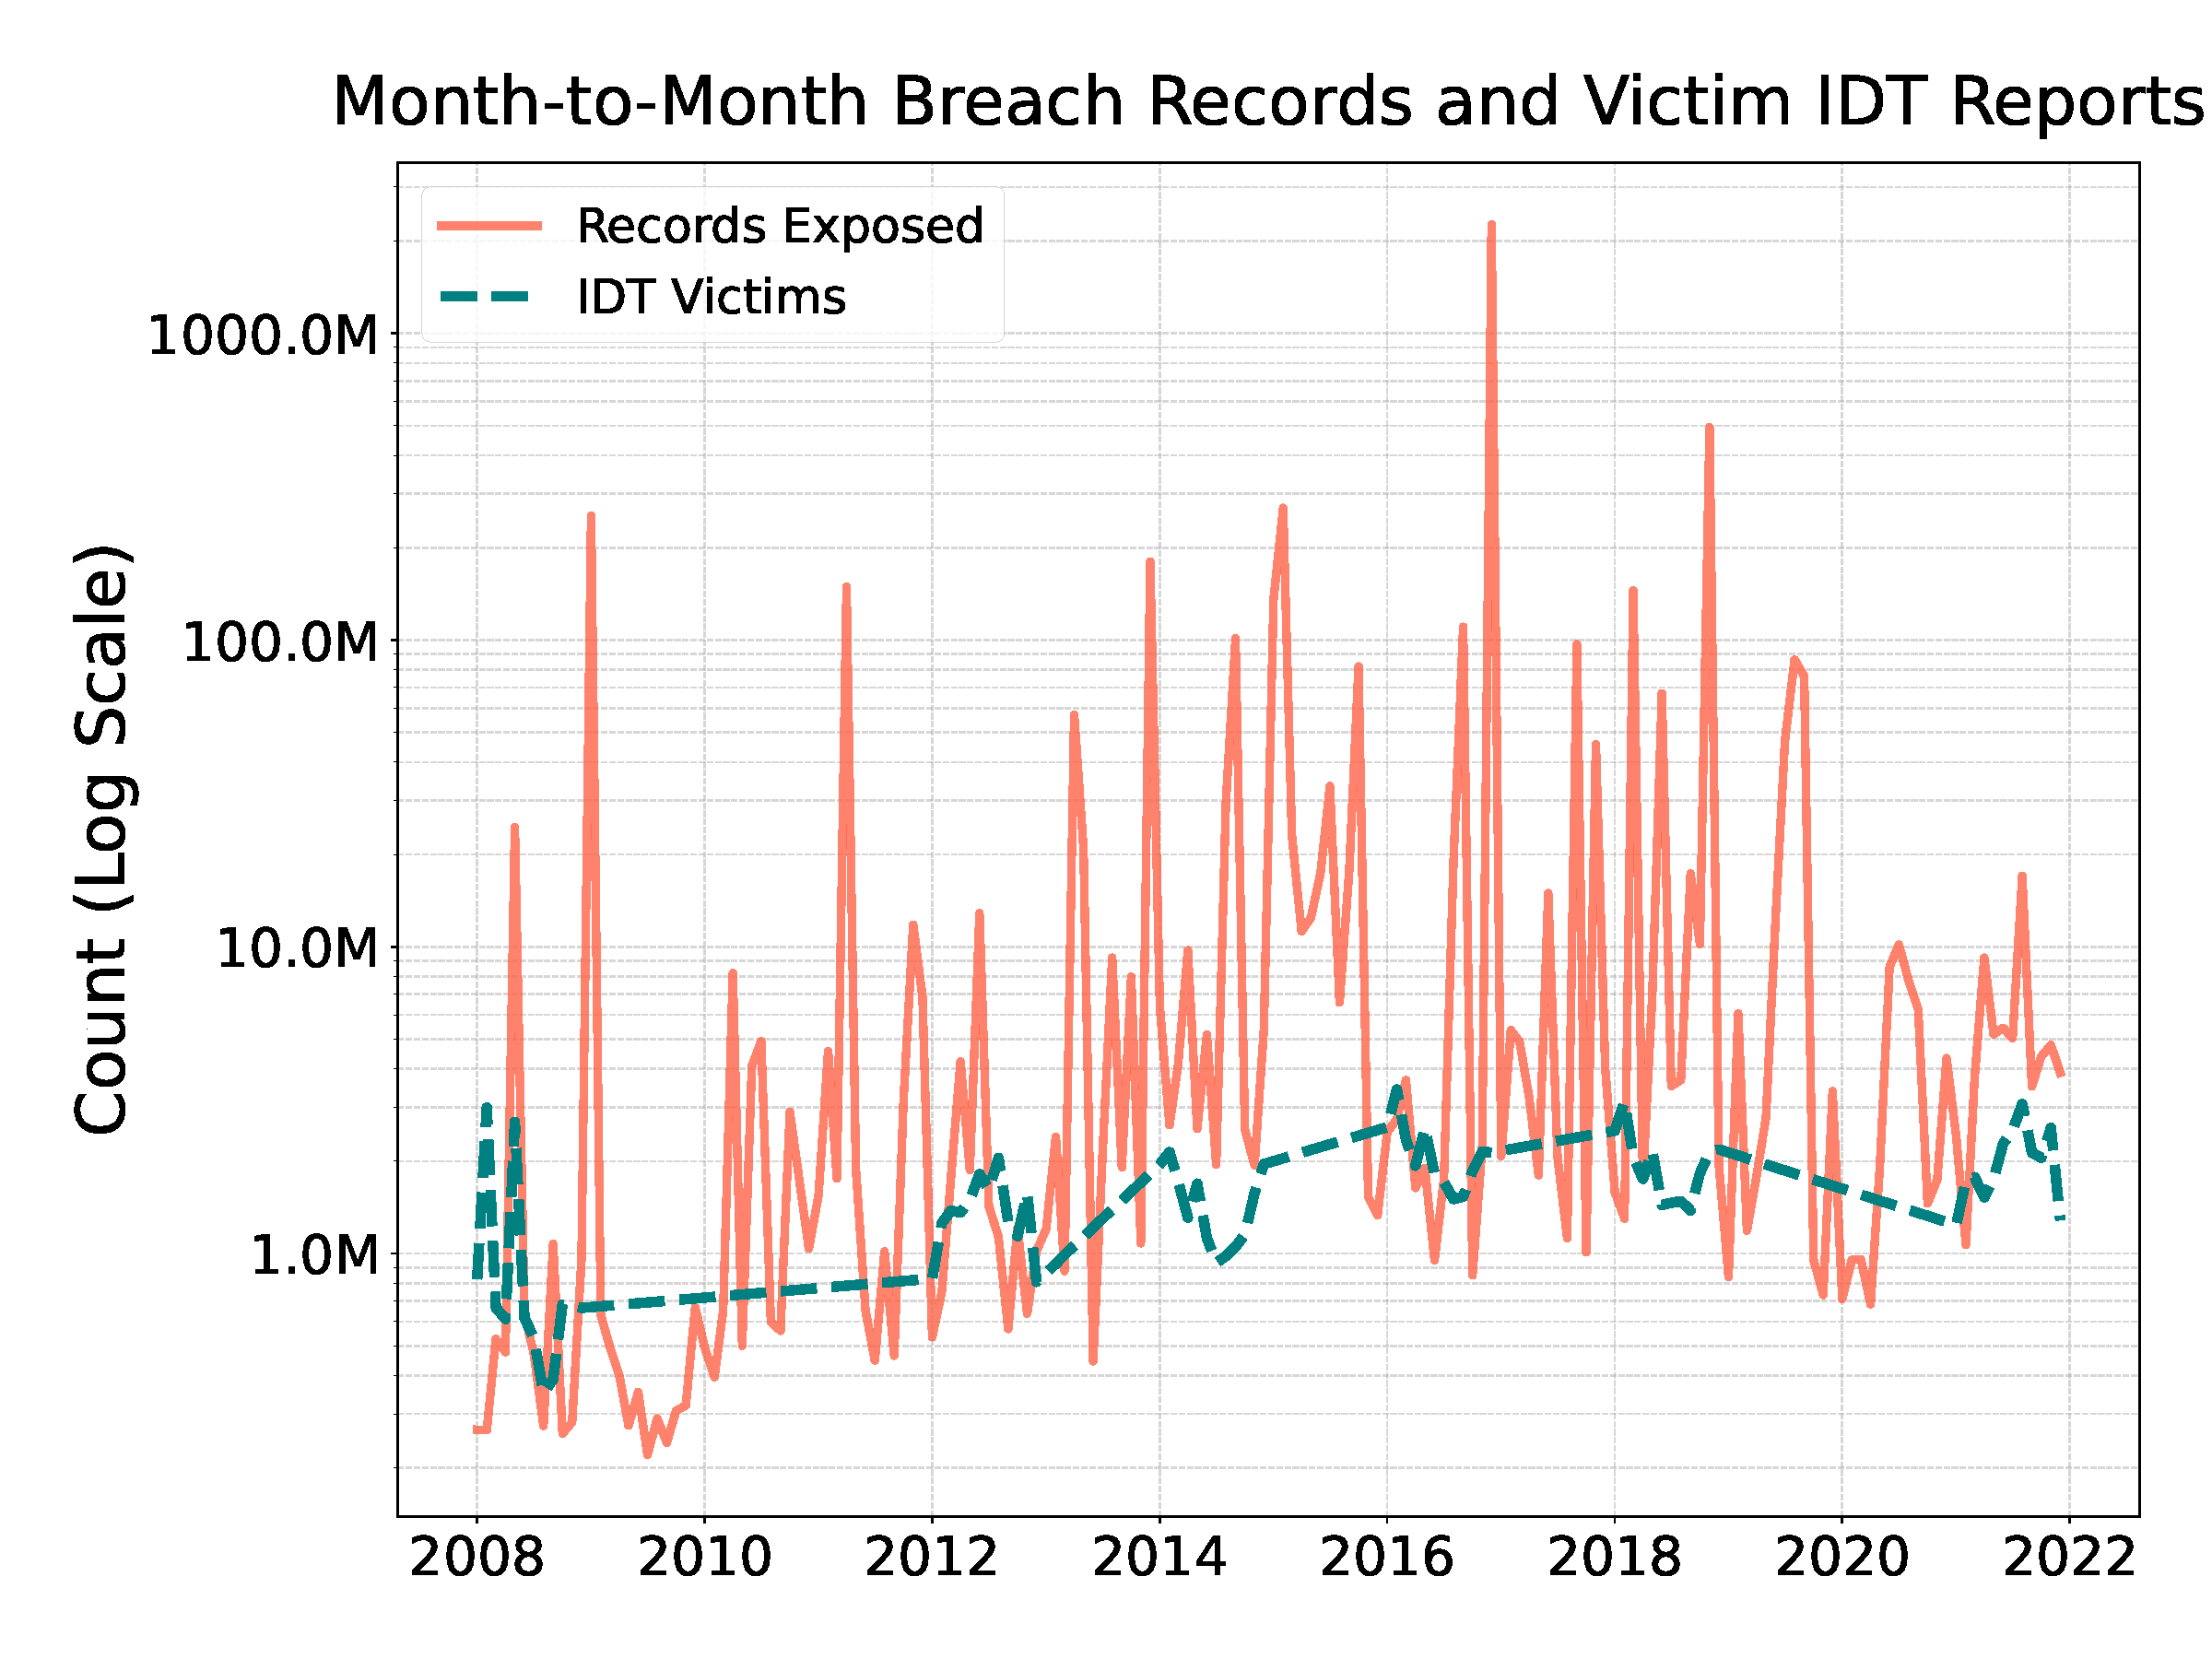
\includegraphics[width=\textwidth]{figures/part5/overlay.pdf}
        \caption{Estimated number of unique individuals compromised (saturation model PRC) and number of reported IDT victims (ITS)}.
        \label{fig:saturation_fig5}
    \end{minipage}
    \hfill 
    % Second Figure
    \begin{minipage}[t]{0.32\textwidth}
        \centering
        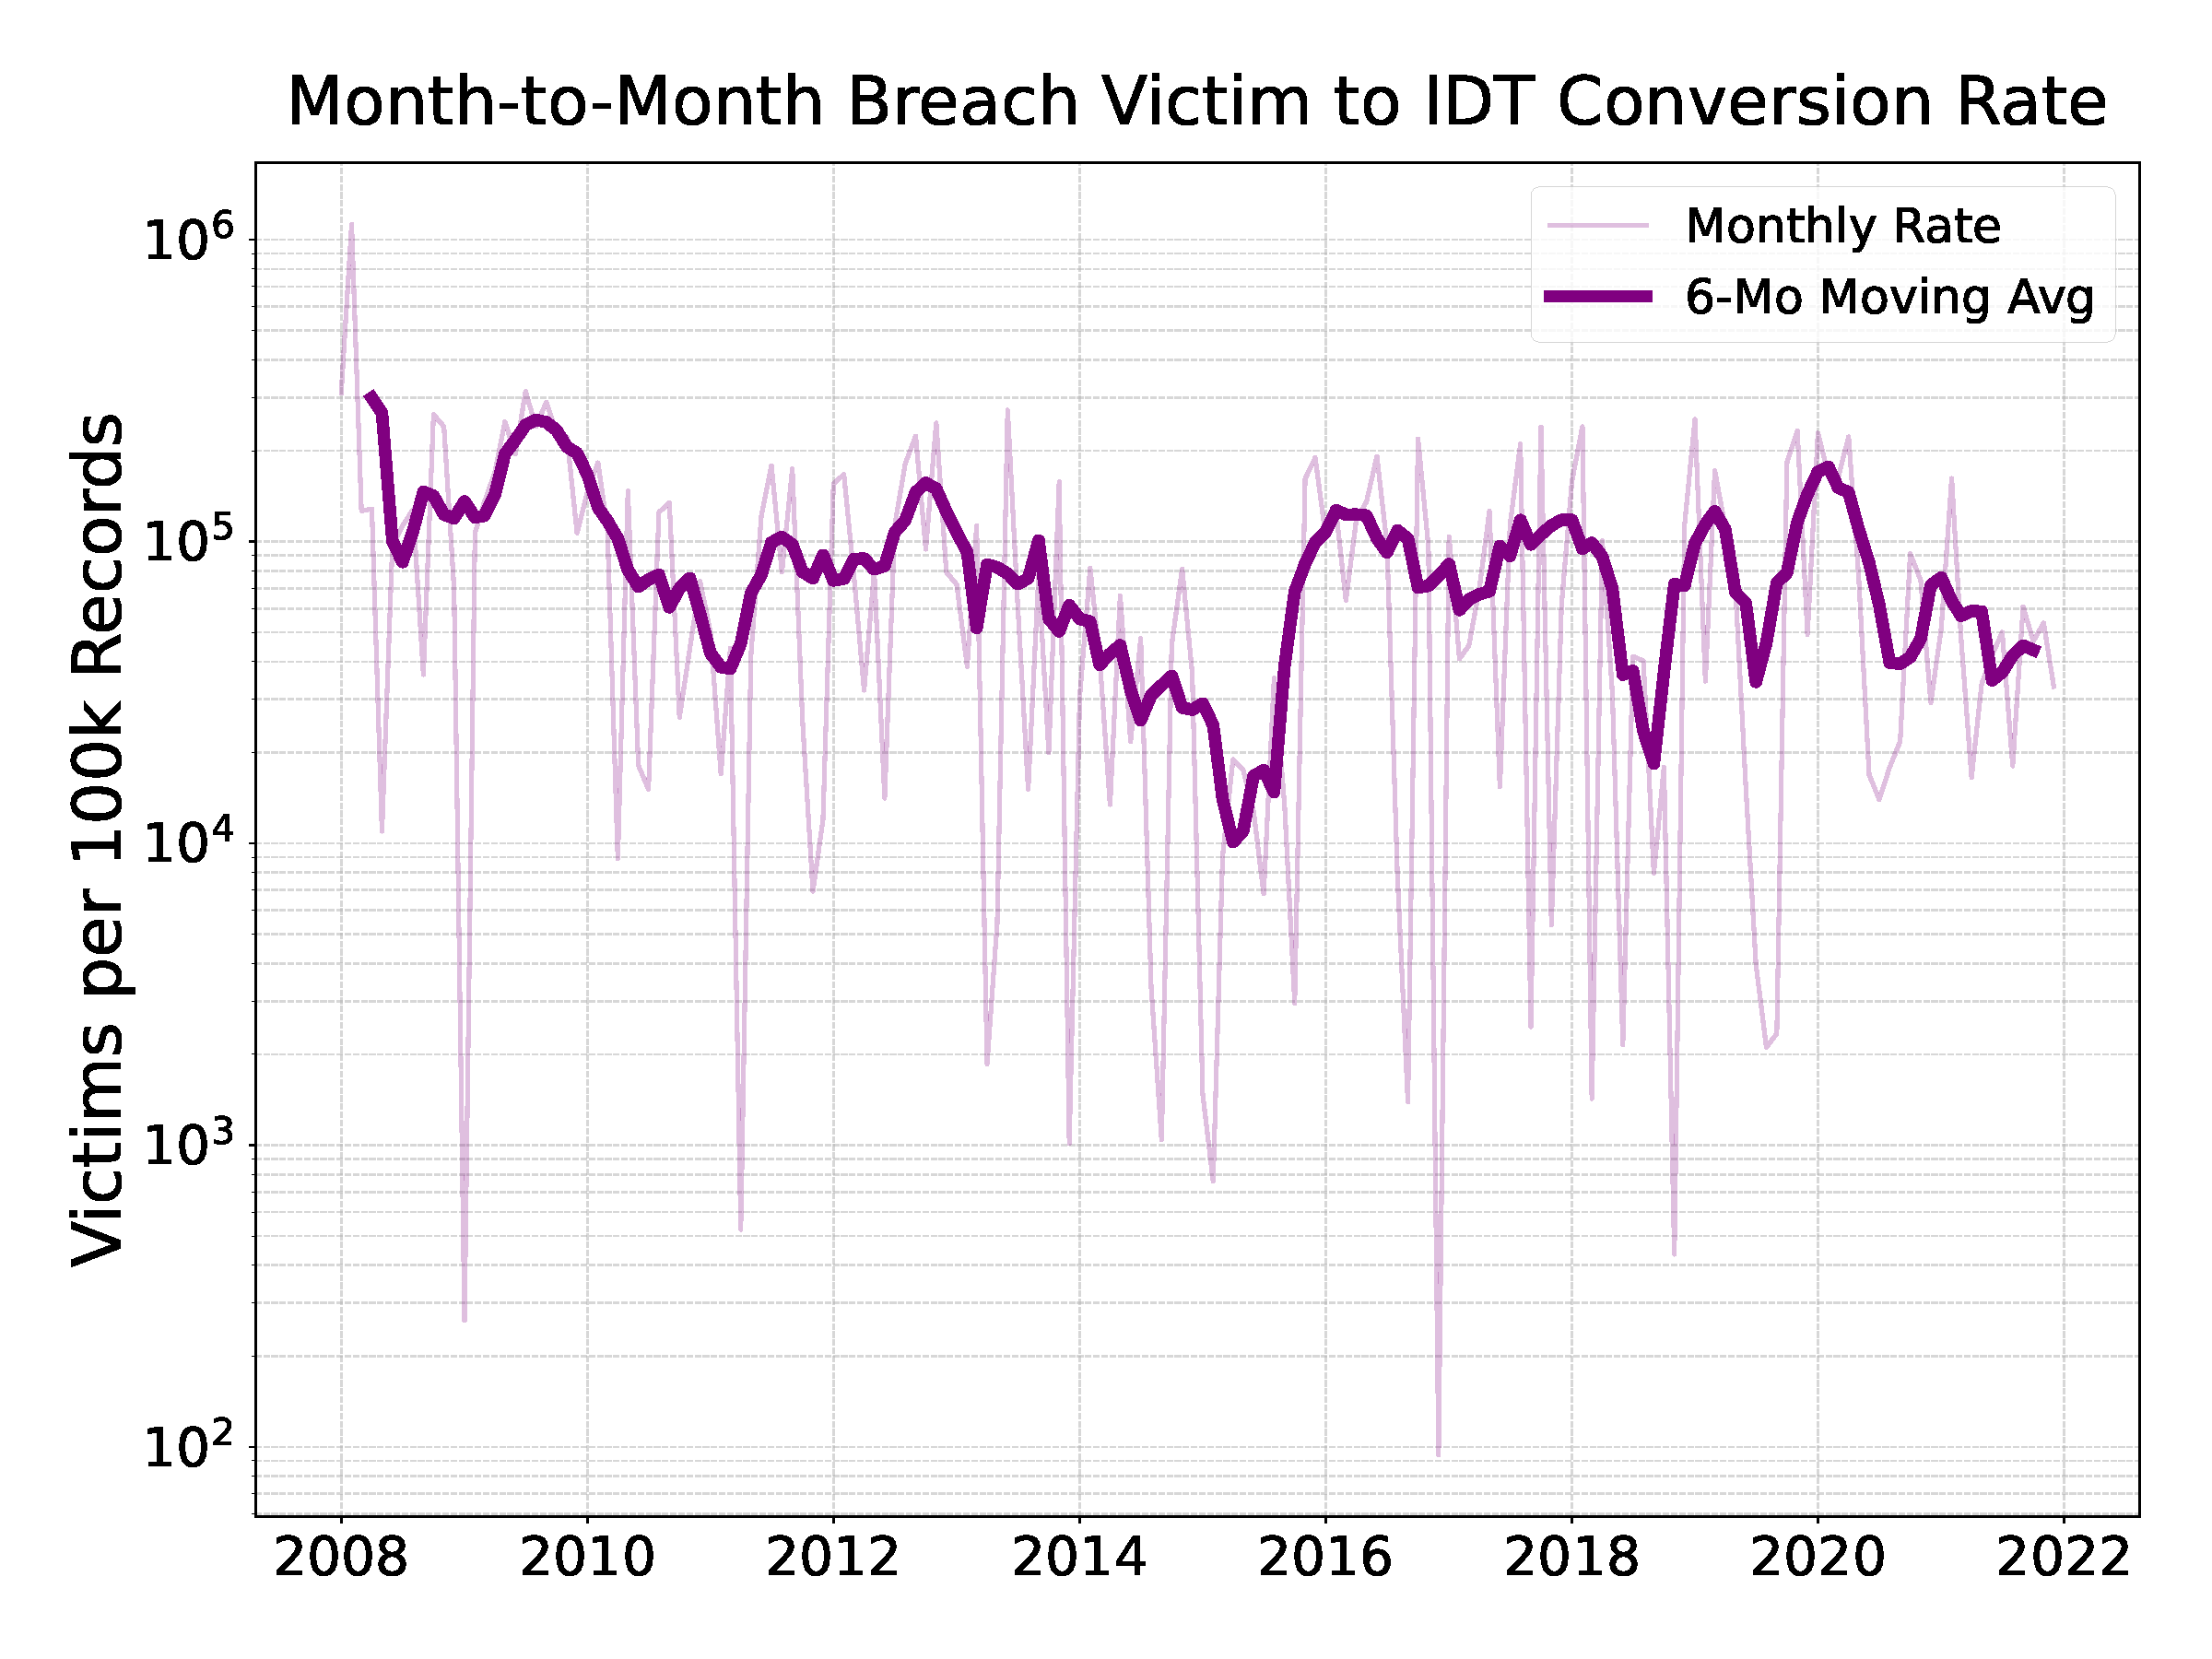
\includegraphics[width=\textwidth]{figures/part5/conversion_rate.pdf}
        \caption{Saturation model conversion rates from data being breached to becoming an IDT victim.}
        \label{fig:saturation_conversion_rate}
    \end{minipage}
    \hfill
    % Third Figure
    \begin{minipage}[t]{0.32\textwidth}
        \centering
        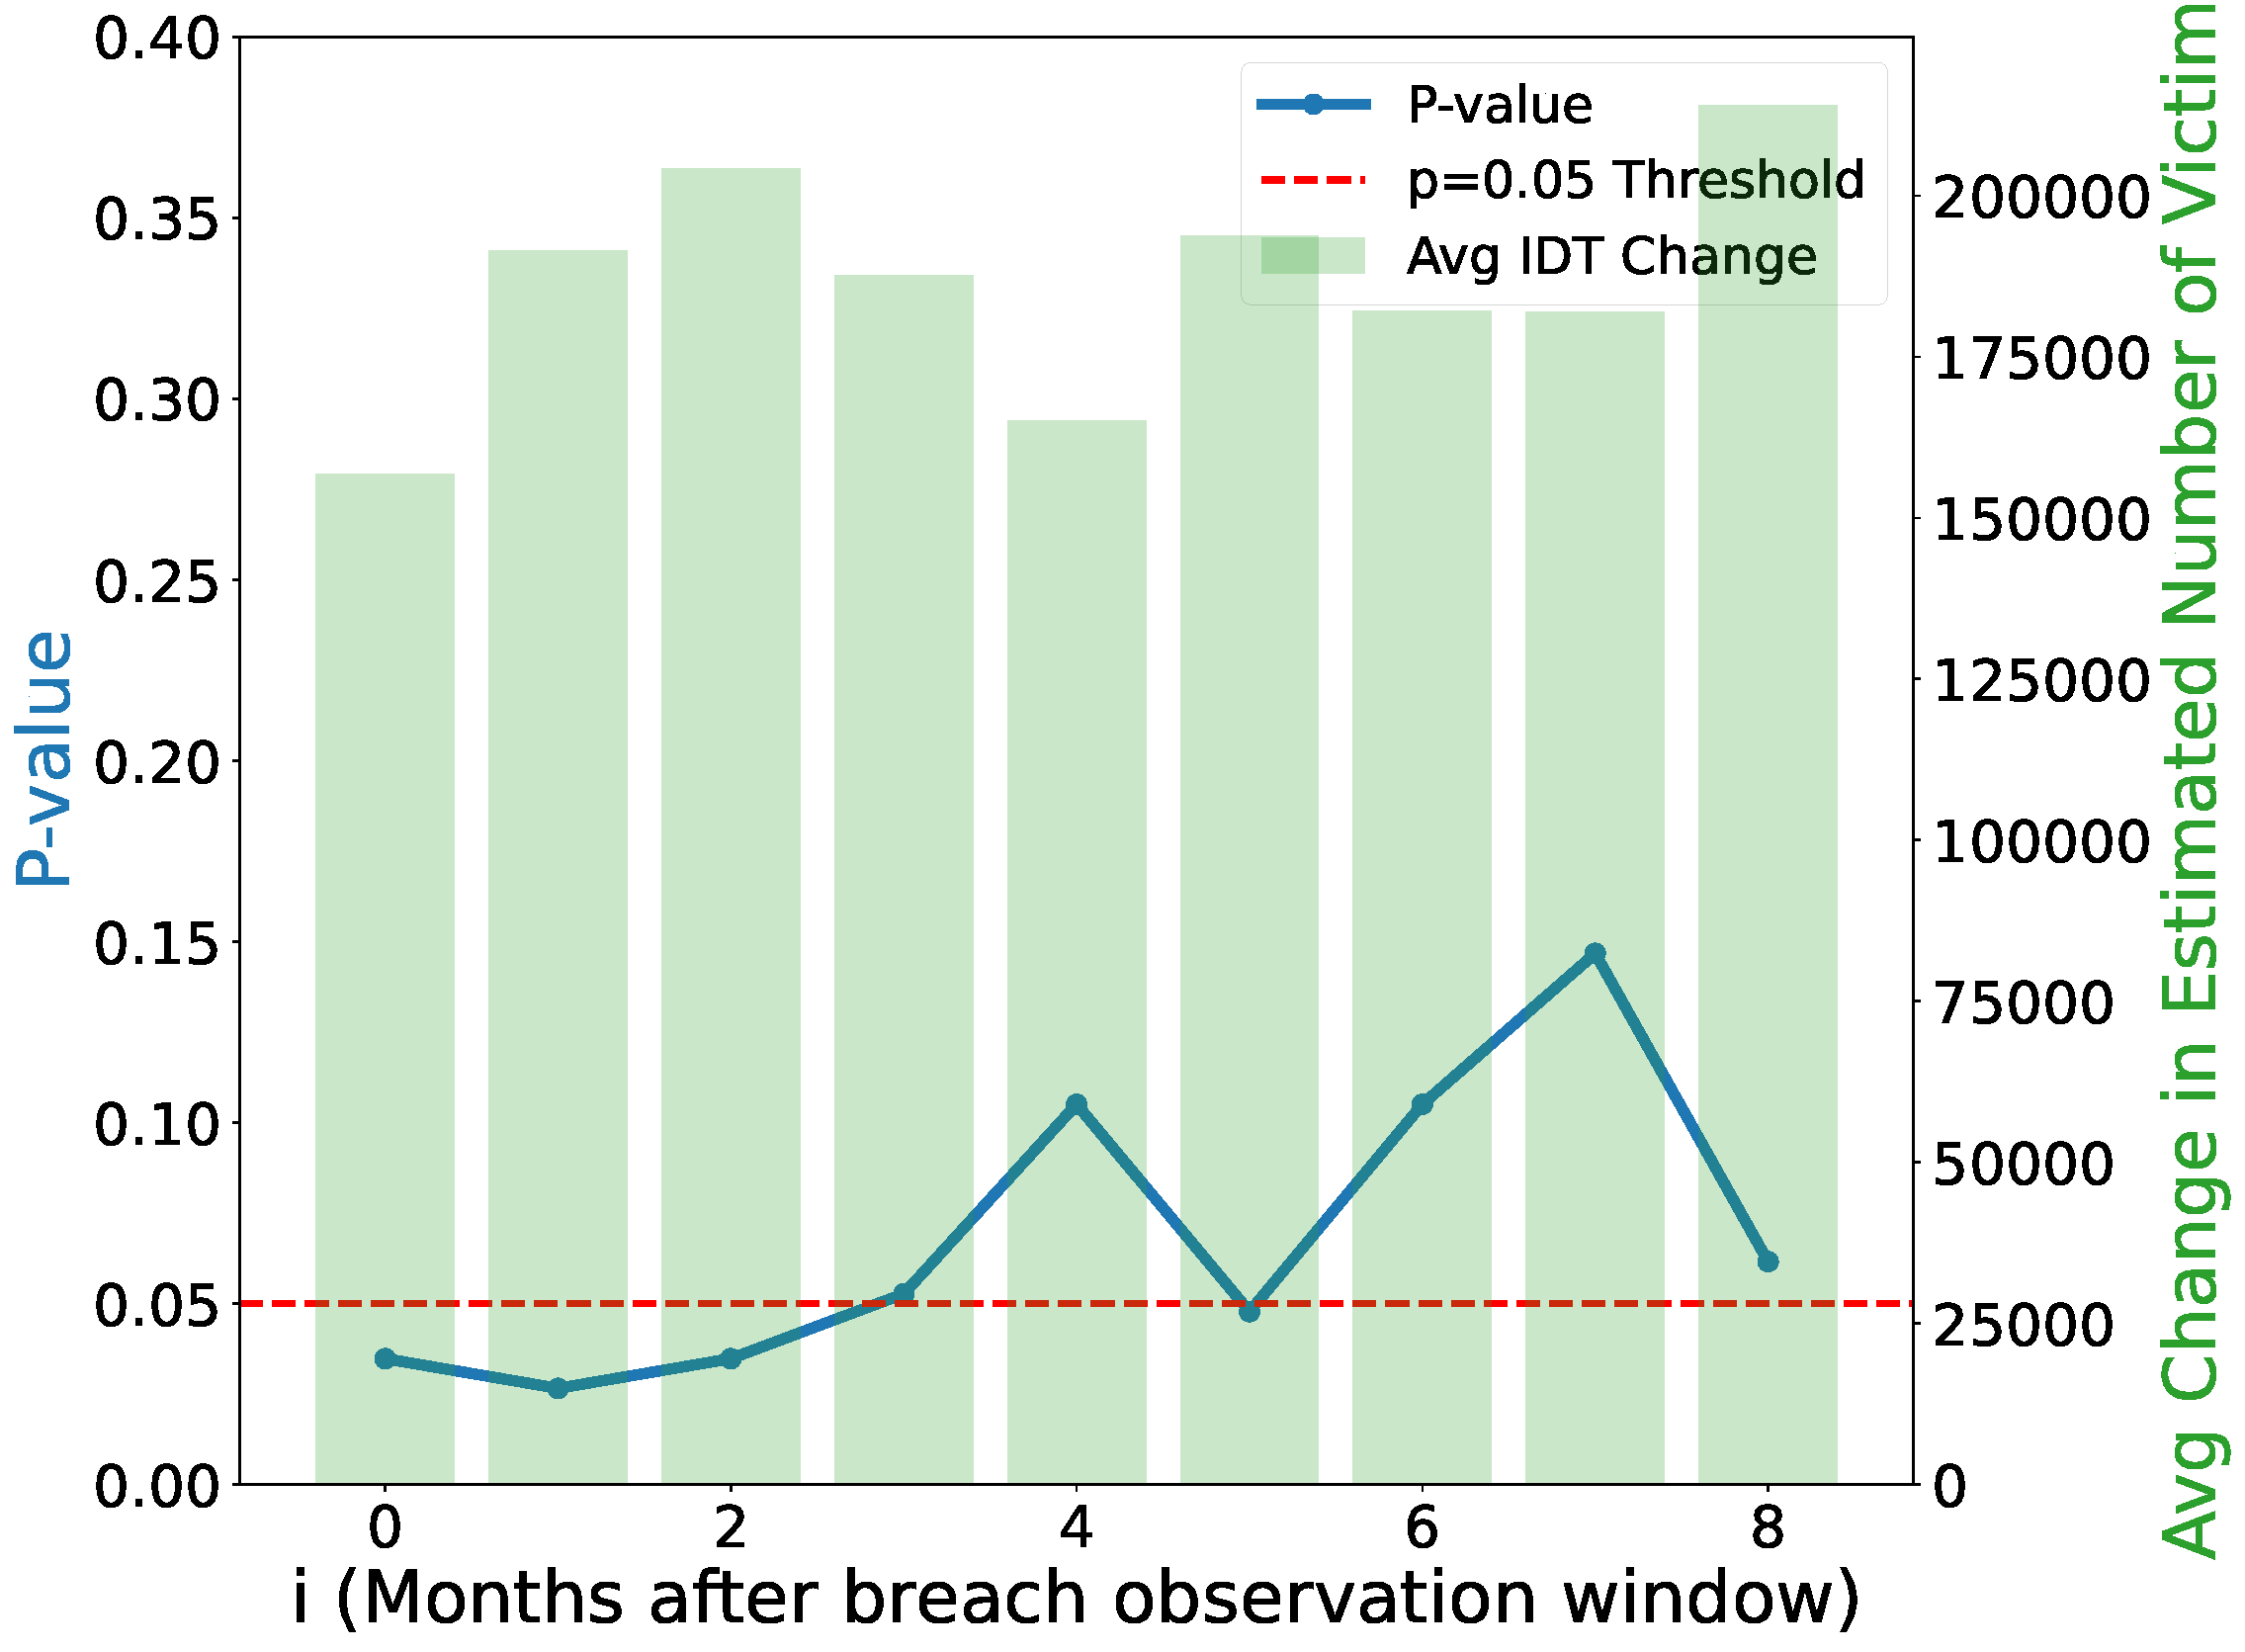
\includegraphics[width=\textwidth]{figures/part6/longitudinal_sweep_saturation_model.pdf}
        \caption{Wilcoxon signed-rank test results for the saturation model PRC data breach chronology data.}
        \label{fig:wilcoxon_sat}
    \end{minipage}
\end{figure}
